\chapter{Preliminaries on Tensor CP decomposition } 
\label{chapter-linear} 

This chapter explains in detail the linear dimensionality reduction method used in this project, tensor canonical polyadic (CP) decomposition, a higher-order generalization of principal component analysis (PCA).

\section{PCA}
Principal component analysis (PCA) is the simplest matrix decomposition model. The PCA model can be formulated as an optimization problem. Given a $N$-by-$M$ matrix $\mathbf{X}$ with $N$ variables and $M$ features, we can approximate $\mathbf{X}$ with the product of two orthogonal rank-one matrices:
\begin{align}
    \mathbf{X} \approx \mathbf{U}\mathbf{V}^T = \sum_{r=1}^R u_r \circ v_r,
\end{align}
where $\circ$ denotes the outer product operator. The equivalent element-wise formulation of the PCA model is
\begin{align}
\label{pca}
    x_{i j} \approx \sum^R_{r = 1} u_i^r v_j^r.
\end{align}
With PCA, the dimensionality of the original matrix can be reduced from from $N$-by-$M$ to $N$-by-$R$. This can be illustrated with the diagram below
\begin{figure}[H]
    \centering
        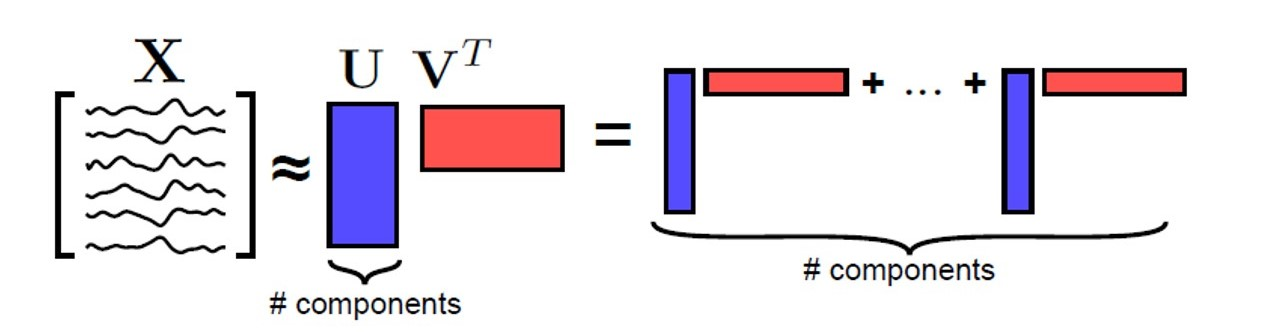
\includegraphics[width=0.7\textwidth]{figures/linear/pca.jpg}
        \caption{Illustration for PCA. (Adapted from (\cite{williams_unsupervised_2018}))}
    \end{figure} 

\begin{itemize}
    \item maximize variance:
\begin{maxi}|l|
  {\mathbf{V}}{\|\mathbf{X}\mathbf{V}\mathbf{V}^T\|_F^2}{}{}
  \addConstraint{\mathbf{V}\text{ orthonormal}}
 \end{maxi}
 \item minimize residuals:
 \begin{mini}|l|
  {\mathbf{U},\mathbf{V}}{\|\mathbf{X} - \mathbf{U}\mathbf{V}^T\|_F^2}{}{}
  \addConstraint{\mathbf{U,V}\text{ orthogonal}}
 \end{mini}
 \begin{rmk}
 Note that without the constraint of $\mathbf{U},\mathbf{V}$ being orthogonal, PCA has infinite number of solutions since
 $\mathbf{U}\mathbf{V}^T = \mathbf{U}F^{-1} F\mathbf{V}^T = \mathbf{U}^\prime \mathbf{V}^{\prime T}.$
 \end{rmk}
\end{itemize}

\par When the data has a non-negative constraint, non-negative matrix factorization (NMF) is used. In NMF, the second part of the optimization becomes the following instead:
 \begin{mini}|l|
  {\mathbf{U},\mathbf{V}}{\|\mathbf{X} - \mathbf{U}\mathbf{V}^T\|_F^2}{}{}
  \addConstraint{\mathbf{U}\geq 0, \mathbf{V} \geq 0.}
 \end{mini}

\section{Higher-order generalization of PCA: tensor CP decomposition}
The main references for this section are  (\cite{williams_unsupervised_2018}),
(\cite{kolda_tensor_2009}), and (\cite{hong_generalized_2020}).

Tensor  canonical polyadic (CP) decomposition generalizes PCA from matrices to higher-order tensors.
\begin{defn}[Tensor norm]
The \underline{norm of tensor} $\mathcal{X} \in \RR^{I_1 \times I_2\times\cdots I_N}$ is
\begin{align}
    \norm{\mathcal{X}} = \sqrt{\sum_{i_1 = 1}^{I_1}\sum_{i_2 = 1}^{I_2}\cdots \sum_{i_N = 1}^{I_N} x_{i_1 i_2 \dots i_N}^2 }.
\end{align}
\end{defn}

\begin{defn}[Rank-one tensors]
An $N$-way tensor $\mathcal{X} \in \RR^{I_1 \times I_2\times\cdots I_N}$ is \underline{rank-one} if it can be written as the outer product of $N$ vectors, that is,
\begin{align}
    \mathcal{X} = \vec{a}^{(1)}\circ \vec{a}^{(2)} \circ \cdots \circ \vec{a}^{(N)}
\end{align}
\end{defn}

Analogous to PCA, tensor CP decomposition aims to approximate the original tensor by a sum of rank-one tensors, each of which can then be written as the outer product of $N$ vectors. Given a $3$-way tensor $\mathcal{X} \in \RR^{I\times J\times K}$, the tensor CP decomposition model is formulated as
\begin{align}
    \mathcal{X} \approx [\![ \mathbf{A}, \mathbf{B}, \mathbf{C} ]\!] = \sum_{r=1}^R a_r \circ b_r \circ c_r,
\end{align}
where $R$ is the number of components and $a_r \in \RR^I, b_r \in \RR^J, c_r \in \RR^K$ for $r = 1,\dots, R.$ The element-wise formulation analogous to \ref{pca} is 
\begin{align}
    x_{i j k} \approx \sum_{r=1}^R a_{i r} b_{j r} c_{k r}
\end{align}
for $i = 1,\dots, I, j = 1,\dots, J, k = 1,\dots,K.$

With tensor CP decomposition, we obtain the tensor factors which are analogous to the principle components. This can be illustrated with the diagram below
\begin{figure}[H]
    \centering
        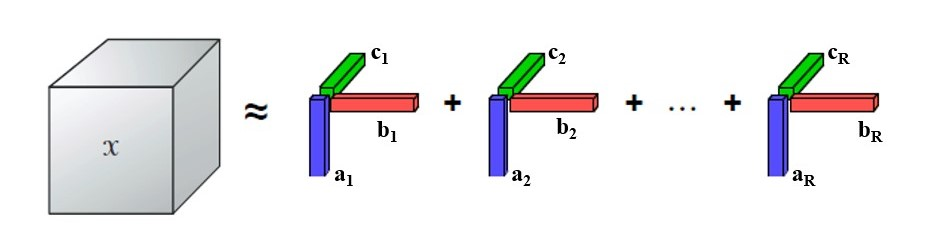
\includegraphics[width=0.7\textwidth]{figures/linear/tca.jpg}
        \caption{Illustration for tensor CP decomposition. (Adapted from (\cite{williams_unsupervised_2018})}
    \end{figure} 
    
The alternating least squares (ALS) method is one of the most common algorithms to compute a tensor CP decomposition with $R$ components. The steps of the ALS are summarized as follows: 
\begin{enumerate}
    \item fix  $\mathbf{B}$ and  $\mathbf{C}$ to solve for $\mathbf{A}$: 
     \begin{equation}
       \min_{\mathbf{A}} \sum_{i j k}\left(x_{i j k} - \sum_l a_{i l} b_{j l} c_{k l}\right)^2
     \end{equation}
    \item fix $\mathbf{A}$ and  $\mathbf{C}$ to solve for  $\mathbf{B}$:
  \begin{align}
       \min_{\mathbf{B}} \sum_{i j k}\left(x_{i j k} - \sum_l a_{i l}  b_{j l} c_{k l}\right)^2
     \end{align}
 \item fix $\mathbf{A}$ and  $\mathbf{B}$ to solve for $\mathbf{C}$: 
 \begin{align}
       \min_{\mathbf{C}} \sum_{i j k}\left(x_{i j k} - \sum_l a_{i l}  b_{j l} c_{k l}\right)^2
     \end{align}
\end{enumerate} 
and repeat the above steps until some convergence criterion is satisfied. 

\section{Demonstrate tensor CP decomposition by using the face image dataset}
As an intuitive demonstration for the tensor CP decomposition method, we apply tensor CP decomposition on face image data with 1000 face images, with each image having dimension $96$-by-$96$. Thus, the face image data are encoded in a $3$-way tensor of dimension $1000$-by-$32$-by-$32$. Using tensor CP decomposition, we obtain the first $5$ tensor components, which intuitively represent the prominent facial features in the face images: 
\begin{figure}[H]
    \centering
        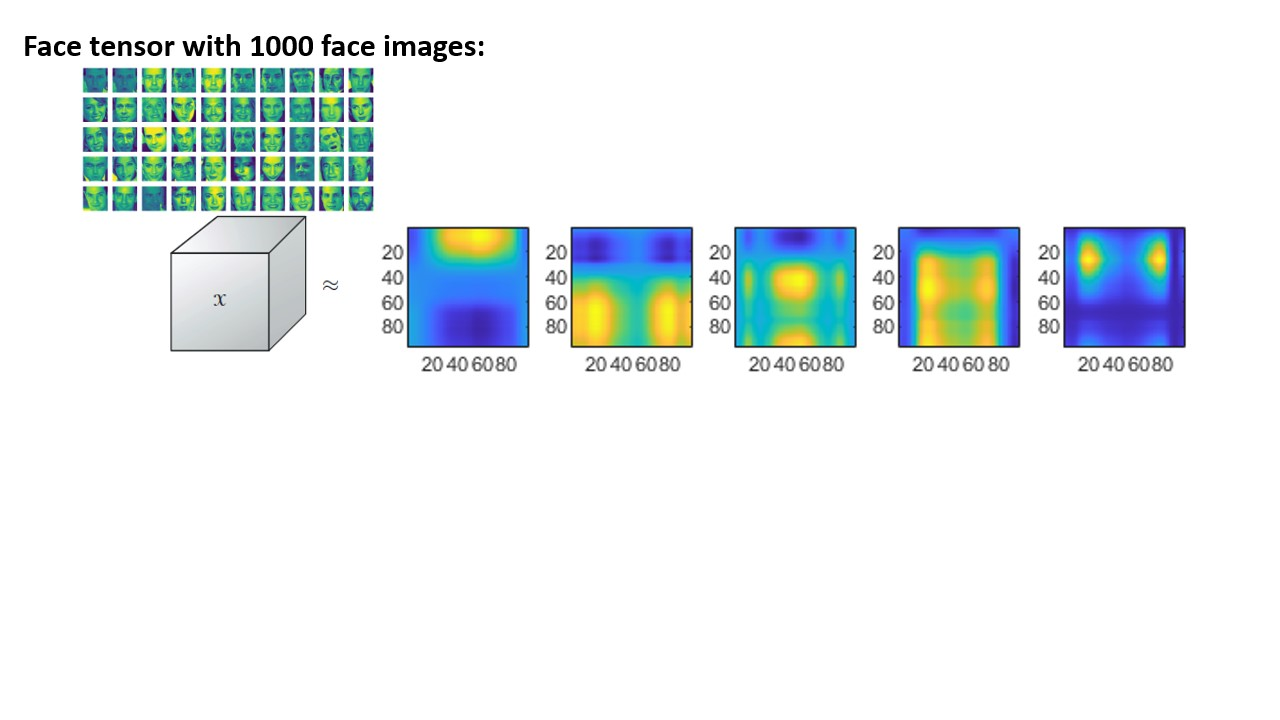
\includegraphics[width=0.7\textwidth]{presentation/Slide2.jpg}
        \caption{First 5 tensor factors for face image data.}
    \end{figure}

By projecting the data onto the first few principal components and apply the $k$-means clustering method, we obtain the following clusters grouped by similar face images: 
\begin{figure}[H]
    \centering
    \begin{subfigure}[b]{0.45\textwidth}
        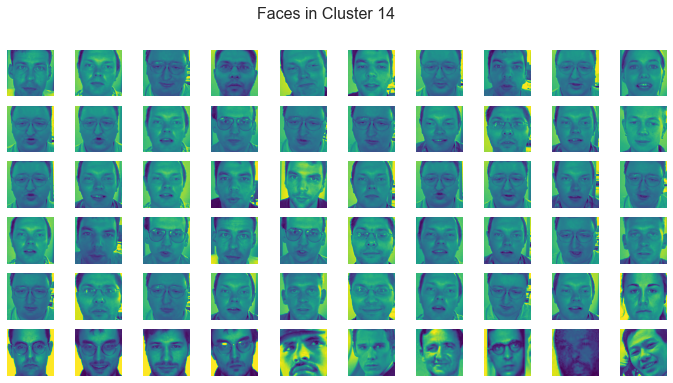
\includegraphics[width=\textwidth]{presentation/figures-face-results/face14.png}
    \end{subfigure}
    \hfill 
    \begin{subfigure}[b]{0.45\textwidth}
        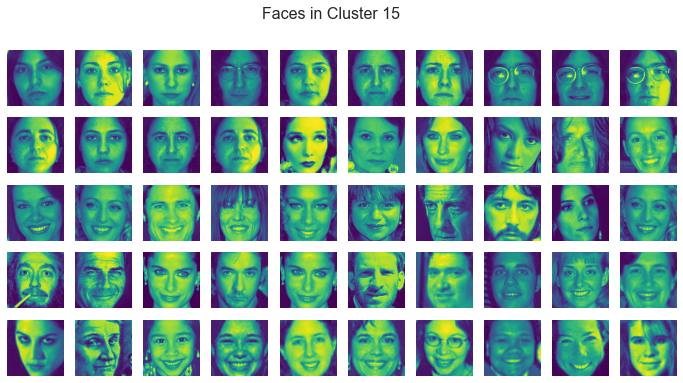
\includegraphics[width=\textwidth]{presentation/figures-face-results/face15.png}
    \end{subfigure}
    \hfill
    \begin{subfigure}[b]{0.45\textwidth}
        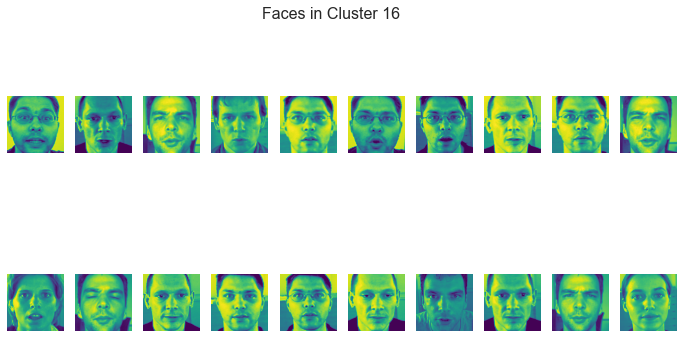
\includegraphics[width=\textwidth]{presentation/figures-face-results/face16.png}
    \end{subfigure}
    \hfill
    \begin{subfigure}[b]{0.45\textwidth}
        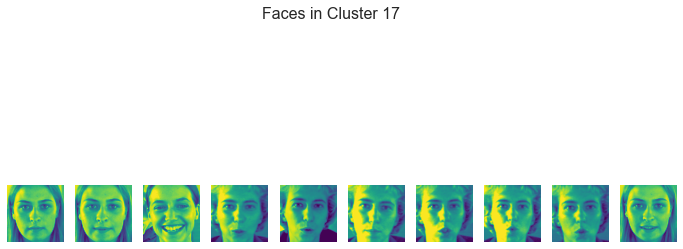
\includegraphics[width=\textwidth]{presentation/figures-face-results/face17.png}
    \end{subfigure}
    \caption{Some arbitrary clusters showing the results of tensor CP decomposition for face data.}
    \end{figure} 
    
\section{Remarks on linear dimensionality reduction}
Linear dimensionality reduction techniques work well when the data lie near a linear subspace of high-dimensional space. They do not work well when the data lie near a non-linear manifold embedded in the high-dimensional space. (\cite{fefferman_testing_2016}) Due to this reason, we introduce the non-linear dimensionality reduction technique of diffusion map in the next chapter. 